%=========================================================================
% (c) 2014, 2015 Josef Lusticky

\section{Ingress traffic processing}\label{sec:linux-ingress}
The traditional way of processing frames from NIC is interrupt-driven~\cite{linux-kernel-networking}.
Each incoming frame is an asynchronous event which raises a hardware interrupt.
Interrupt handlers run asynchronously with either the current interrupt level disabled or with all
interrupts disabled~\cite{lkd2}.
The handlers could interrupt other potentially important code, therefore they need to run as quickly as possible.
Interrupt handlers immediately respond to hardware and perform time-critical actions,
however, other less critical work should be deferred to a later point when interrupts are enabled~\cite{lkd2}.

Upon frame reception, the hardware interrupt handler of the network adpater
performs the following immediate tasks:~\cite{understanding-internals}
\begin{enumerate}
\item Copies the frame into an {\it{sk\_buff}} data structure.
If DMA is used by the device, the kernel needs only to initialise a buffer and pass its descriptors to the driver,
which instructs the device to use DMA.
The received frame is then copied by a DMA transfer.
\item Initialises some of the {\it{sk\_buff}} members for later usage by upper network layers,
notably the {\it{protocol}} member, which identifies the higher-layer protocol handler and will play a major role later.
\item Updates some other parameters private to the device, such as variables for statistical purposes.
\item Signals the kernel about the new frame by scheduling the NET\_RX\_SOFTIRQ softirq for execution.
\end{enumerate}

To keep the execution of the handler as short as possible,
further frame processing is performed later in the NET\_RX\_SOFTIRQ routine.
This softirq routine actually performs an interrupt-related work
not performed in the hardware interrupt handler~\cite{understanding-internals}.
The routine further passes the received frame
to the corresponding L3 protocol handler according to the {\it{protocol}} member of the {\it{skb}}~\cite{lkd2}.
In case of IPv4, this is the {\it{ip\_rcv()}} function described in section~\ref{sec:linux-routing}.
Moreover, the softirq routine is threaded and can run concurrently on different CPUs~\cite{lkd2}.

However, such method of packet processing became insufficient with the emerge of high-speed network cards.
Even a moderately busy interface can handle thousands of packets per second
and per-packet interrupts quickly overwhelm the processor with interrupt-handling work~\cite{low-latency-ethernet-device-polling}.
On the way towards high-speed packet processing on the host CPU,
packet processing in the network stack must have been adapted.

NAPI ("New API", though not so new anymore)
is an interrupt mitigation mechanism used with network devices~\cite{reworking-napi}.
NAPI mixes interrupts with polling and gives higher performance under high traffic load
than the old approach, by reducing significantly the load on the CPU~\cite{understanding-internals}.

%=========================================================================
% (c) 2014, 2015 Josef Lusticky

\subsection{NAPI}\label{subsec:linux-ingress-napi}
NAPI was first introduced during the Linux kernel 2.5 development cycle as
an extension to the device driver packet processing framework,
which is designed to improve the performance of high-speed networking~\cite{linux-foundation-napi}.

A NAPI-compliant device driver must implement a {\it{poll()}} function used by the kernel to fetch the received frames.
The first frame received causes a hardware interrupt and its handler to run as usual.
In the handler, however, the driver disables interrupts from the device
and calls the {\it{netif\_rx\_schedule()}} function.
This function adds the device to the kernel's {\it{poll\_list}} and schedules the NET\_RX\_SOFTIRQ routine.
From now on, the task of delivering more incoming frames from
the device's queue is delegated to the kernel~\cite{understanding-internals}.

In the NET\_RX\_SOFTIRQ routine, the kernel iterates over the polll\_list and keeps calling
the {\it{poll()}} function of the device driver to fetch the frames from the device's ingress queue (implemented as a ring buffer).
The kernel fetches the packets and passes them to the higher-layer protocol handler for further processing~\cite{linux-kernel-networking}.
The {\it{poll()}} function is called with a maximum number
of packets ({\it{budget}}) it is allowed to feed into the kernel.
It should process up to that many packets and return~\cite{reworking-napi}.
Figure~\ref{fig:linux-napi-workflow} shows the NAPI workflow described above.

\begin{figure}
	\centering
	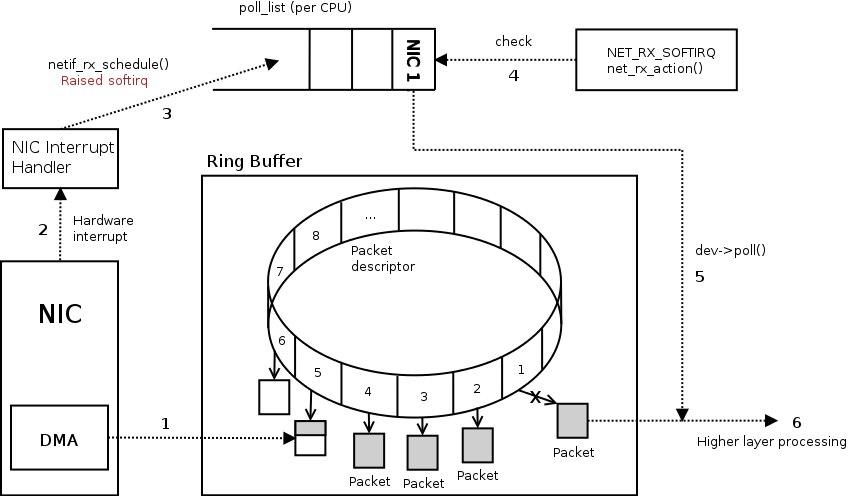
\includegraphics[width=15cm,keepaspectratio]{fig/napi-workflow.png}
	\caption{NAPI workflow}
	\label{fig:linux-napi-workflow}
\end{figure}

When the kernel is ready to deal with more packets, the {\it{poll()}} function of the next device
in the {\it{poll\_list}} will be called.
The scheduled devices are probed in a round-robin manner.
The total number of packets fetched from devices in the {\it{poll\_list}} is limited.
If it was not sufficient to serve all devices in the {\it{poll\_list}} and the kernel should release the CPU,
the devices have to wait for the next NET\_RX\_SOFTIRQ run~\cite{understanding-internals}.
The softirq NET\_RX\_SOFTIRQ processing for NAPI-compliant drivers
is implement by the {\it{net\_rx\_action()}} function defined in {\it{net/core/dev.c}}~\cite{kernel-source}.
The function overview is shown in figure~\ref{fig:linux-softirq-napi}.

\begin{figure}
	\centering
	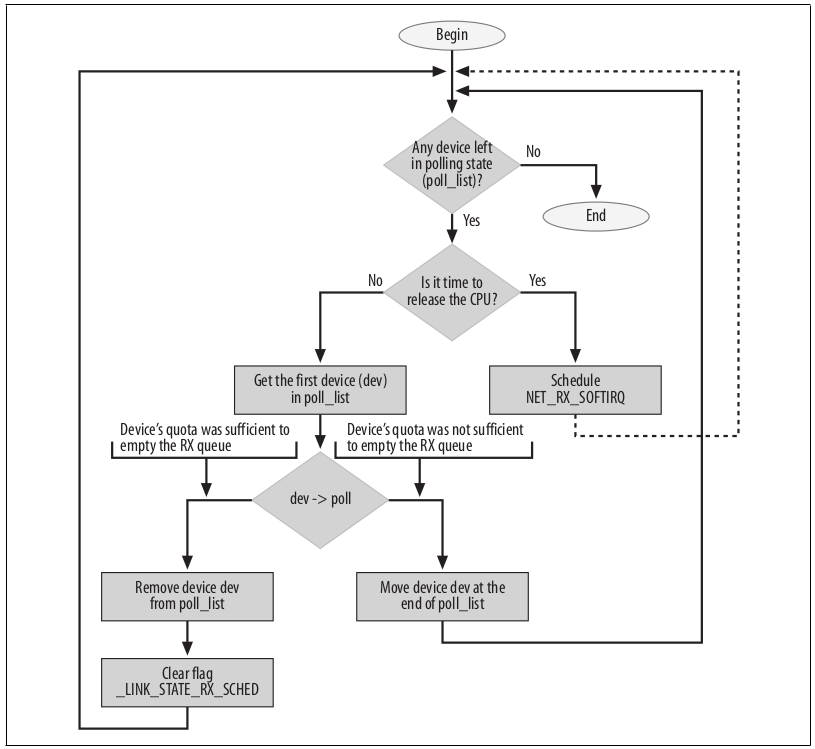
\includegraphics[width=14.5cm,keepaspectratio]{fig/net_rq_softirq.png}
	\caption{Softirq NAPI routine {\it{net\_rx\_action}} (source:~\cite{understanding-internals})}
	\label{fig:linux-softirq-napi}
\end{figure}

When a device driver uses NAPI, it is up to
the driver to implement any congestion control mechanism.
This is because ingress frames are kept in the NIC's memory or in the receive ring buffer managed by the driver,
and the kernel cannot keep track of traffic congestion~\cite{understanding-internals}.
When the host becomes congested, the packets are lost because of not enough space in the ring buffer.
The packets that are going to be lost are not fed into the network stack, so they take no CPU time~\cite{haifux-lecture}.

When a device cannot clear out its ingress queue in a single poll,
it has to wait until the next call.
The kernel keeps calling the driver's {\it{poll()}} function until
it empties the device's ingress queue out~\cite{understanding-internals}.
At that point, there is no need anymore for polling.
The device is removed from the {\it{poll\_list}}
and the device driver can re-enable interrupt notifications for the device~\cite{understanding-internals}.
Nowadays, almost every driver supports the NAPI feature~\cite{linux-kernel-networking}.

NAPI reduces interrupt load on the system and lowers the CPU utilisation under heavy load,
but it increases latency as packets are not processed as quickly~\cite{linux-foundation-napi}.
User-space applications that need the lowest
possible latency and are willing to pay a cost of higher CPU utilisation,
can use a capability for busy polling on sockets (called Low Latency Sockets), which was added in kernel 3.11~\cite{linux-kernel-networking}.
Low Latency Sockets eliminate the cost of the interrupt and context switch
and provide latency very close to the hardware latency~\cite{intel-lls}.

In addition to NAPI, various offload engines were designed to take over some responsibilities of the networking code
and implement them in hardware.


%=========================================================================
% (c) 2014, 2015 Josef Lusticky

\subsection{Receive offloads}\label{subsec:linux-ingress-offloads}
Network adapter vendors have been adding protocol support to their cards.
This support can vary from the simple (checksumming of packets, for example)
through to full TCP/IP implementations~\cite{linux-and-tcp-offload-engines}.

To mitigate CPU load spent on TCP overhead completely, the TCP Offload Engine (TOE) is implemented in several NICs.
TOE features a full TCP/IP implementation in adapter, including the TCP connection management.
However, Linux has never supported the TOE features of any network cards~\cite{linux-and-tcp-offload-engines}.
Vendors have made modifications to the Linux kernel to support TOE,
and these changes have been submitted for kernel inclusion but were rejected~\cite{linux-foundation-toe}. 

Linux kernel engineers currently feel that the full network stack offload
that TOE provides has little merit~\cite{linux-foundation-toe}.
TOE shorts out much of the Linux networking code, described in the previous sections.
In the process, it cuts out features like Netfilter, traffic control, and more.
The Linux networking stack is easy to fix when a bug or security issue comes up~\cite{linux-and-tcp-offload-engines}.
If a security problem turns up in a TOE adapter, instead, there is very little which can be done to fix it.
Linux engineers claim that 100~Mbps TOE adapters
(which used to be the bleeding-edge high speed)
are now slower than the Linux networking stack.
So any performance advantage from TOE is a temporary thing, but once the TOE's code is merged, it must be supported.
As a result of this, TOE support might become a long-term maintenance burden~\cite{linux-and-tcp-offload-engines}.

Although inclusion of TOE support was rejected, there are ways to obtain TOE's performance without
necessitating stateful support in the cards~\cite{linux-and-tcp-offload-engines}.
Everything that is worthwhile can be done with stateless offloads.
One of the simplest stateless offload technique is computing checksums in hardware.
With receive (Rx) checksum offload, IP, TCP and UDP checksums are checked in the hardware of the NIC upon frame reception.

While checksum offload provides some performance improvement,
a large portion of per-packet processing overhead remains.
Each packet is passed through the entire IP stack, as described in section~\ref{sec:linux-ip}.
Dealing with each single packet takes a significant amount of the CPU time, particularly on high-speed Ethernet links that
can produce millions of packets per second.

Given the importance of per-packet overhead, it makes sense to raise the MTU.
However, most connections of interest go across the Internet,
and those are all bound by the lowest MTU in the entire path.
As noted in section~\ref{sec:40gbe-compatibility}, the IEEE has determined no support for frames with MTU larger than 1500.
Protocol-based mechanisms for MTU discovery exist, but they do not work well on the Internet,
because in particular, a lot of firewall setups do not allow them to work~\cite{jls2009-gro}.

If the kernel can not use a larger MTU, it can pretend that it is using a larger MTU.
An optimisation technique to pretend larger MTU is provided by the Large Receive Offload (LRO).
LRO merges packets of the same TCP flow together,
creating one large super-frame, before it is passed to the higher network layers~\cite{jls2009-gro}.
Merging multiple packets and processing them as a single packet
reduces CPU overhead and thus improves performance~\cite{linux-kernel-networking}.
The merging can be done either in the driver or in the hardware.
Even LRO emulation in the driver has performance benefits~\cite{jls2009-gro}.

Since LRO merges everything of the same TCP flow into one large super-frame,
the differences in the headers of these packets are lost~\cite{jls2009-gro}.
If a system is acting as a router, it should not be changing the headers on packets as they pass through,
because it brakes the end-to-end principle and can significantly impact performance~\cite{linux-kernel-networking}.

A generic solution was introduced by the Generic Receive Offload (GRO) to mitigate the problems of LRO.
In GRO, the criteria for which packets can be merged is greatly restricted.
The MAC headers must be identical and only a few TCP or IP headers can differ -
checksums are necessarily different and the Identification field is allowed to increment~\cite{jls2009-gro}.
As a result of these restrictions, merged packets can be later resegmented losslessly
and therefore the GRO feature can be used by a system
acting as a router without braking the end-to-end principle~\cite{jls2009-gro}.
However, GRO still requires the L4 protocol to have its own segmentation support
and it is currently restricted to TCP only~\cite{linux-kernel-networking}.

When using GRO, merging packets of the same flow into one large super-frame must be time-limited.
In combination with NAPI, there is no need for any special waiting code -
the kernel already calls the driver's poll method for new packets occasionally and processes them in batches.
Thus, GRO can simply be performed at NAPI poll time without introducing any additional latency~\cite{jls2009-gro}.
The GRO feature improves network performance
and it deprecated LRO in recent kernels~\cite{linux-kernel-networking}.
Figure~\ref{fig:linux-rcv-offloads} shows comparison of ingress frames processing
with and without the above described offload mechanisms.

\begin{figure}
	\centering
	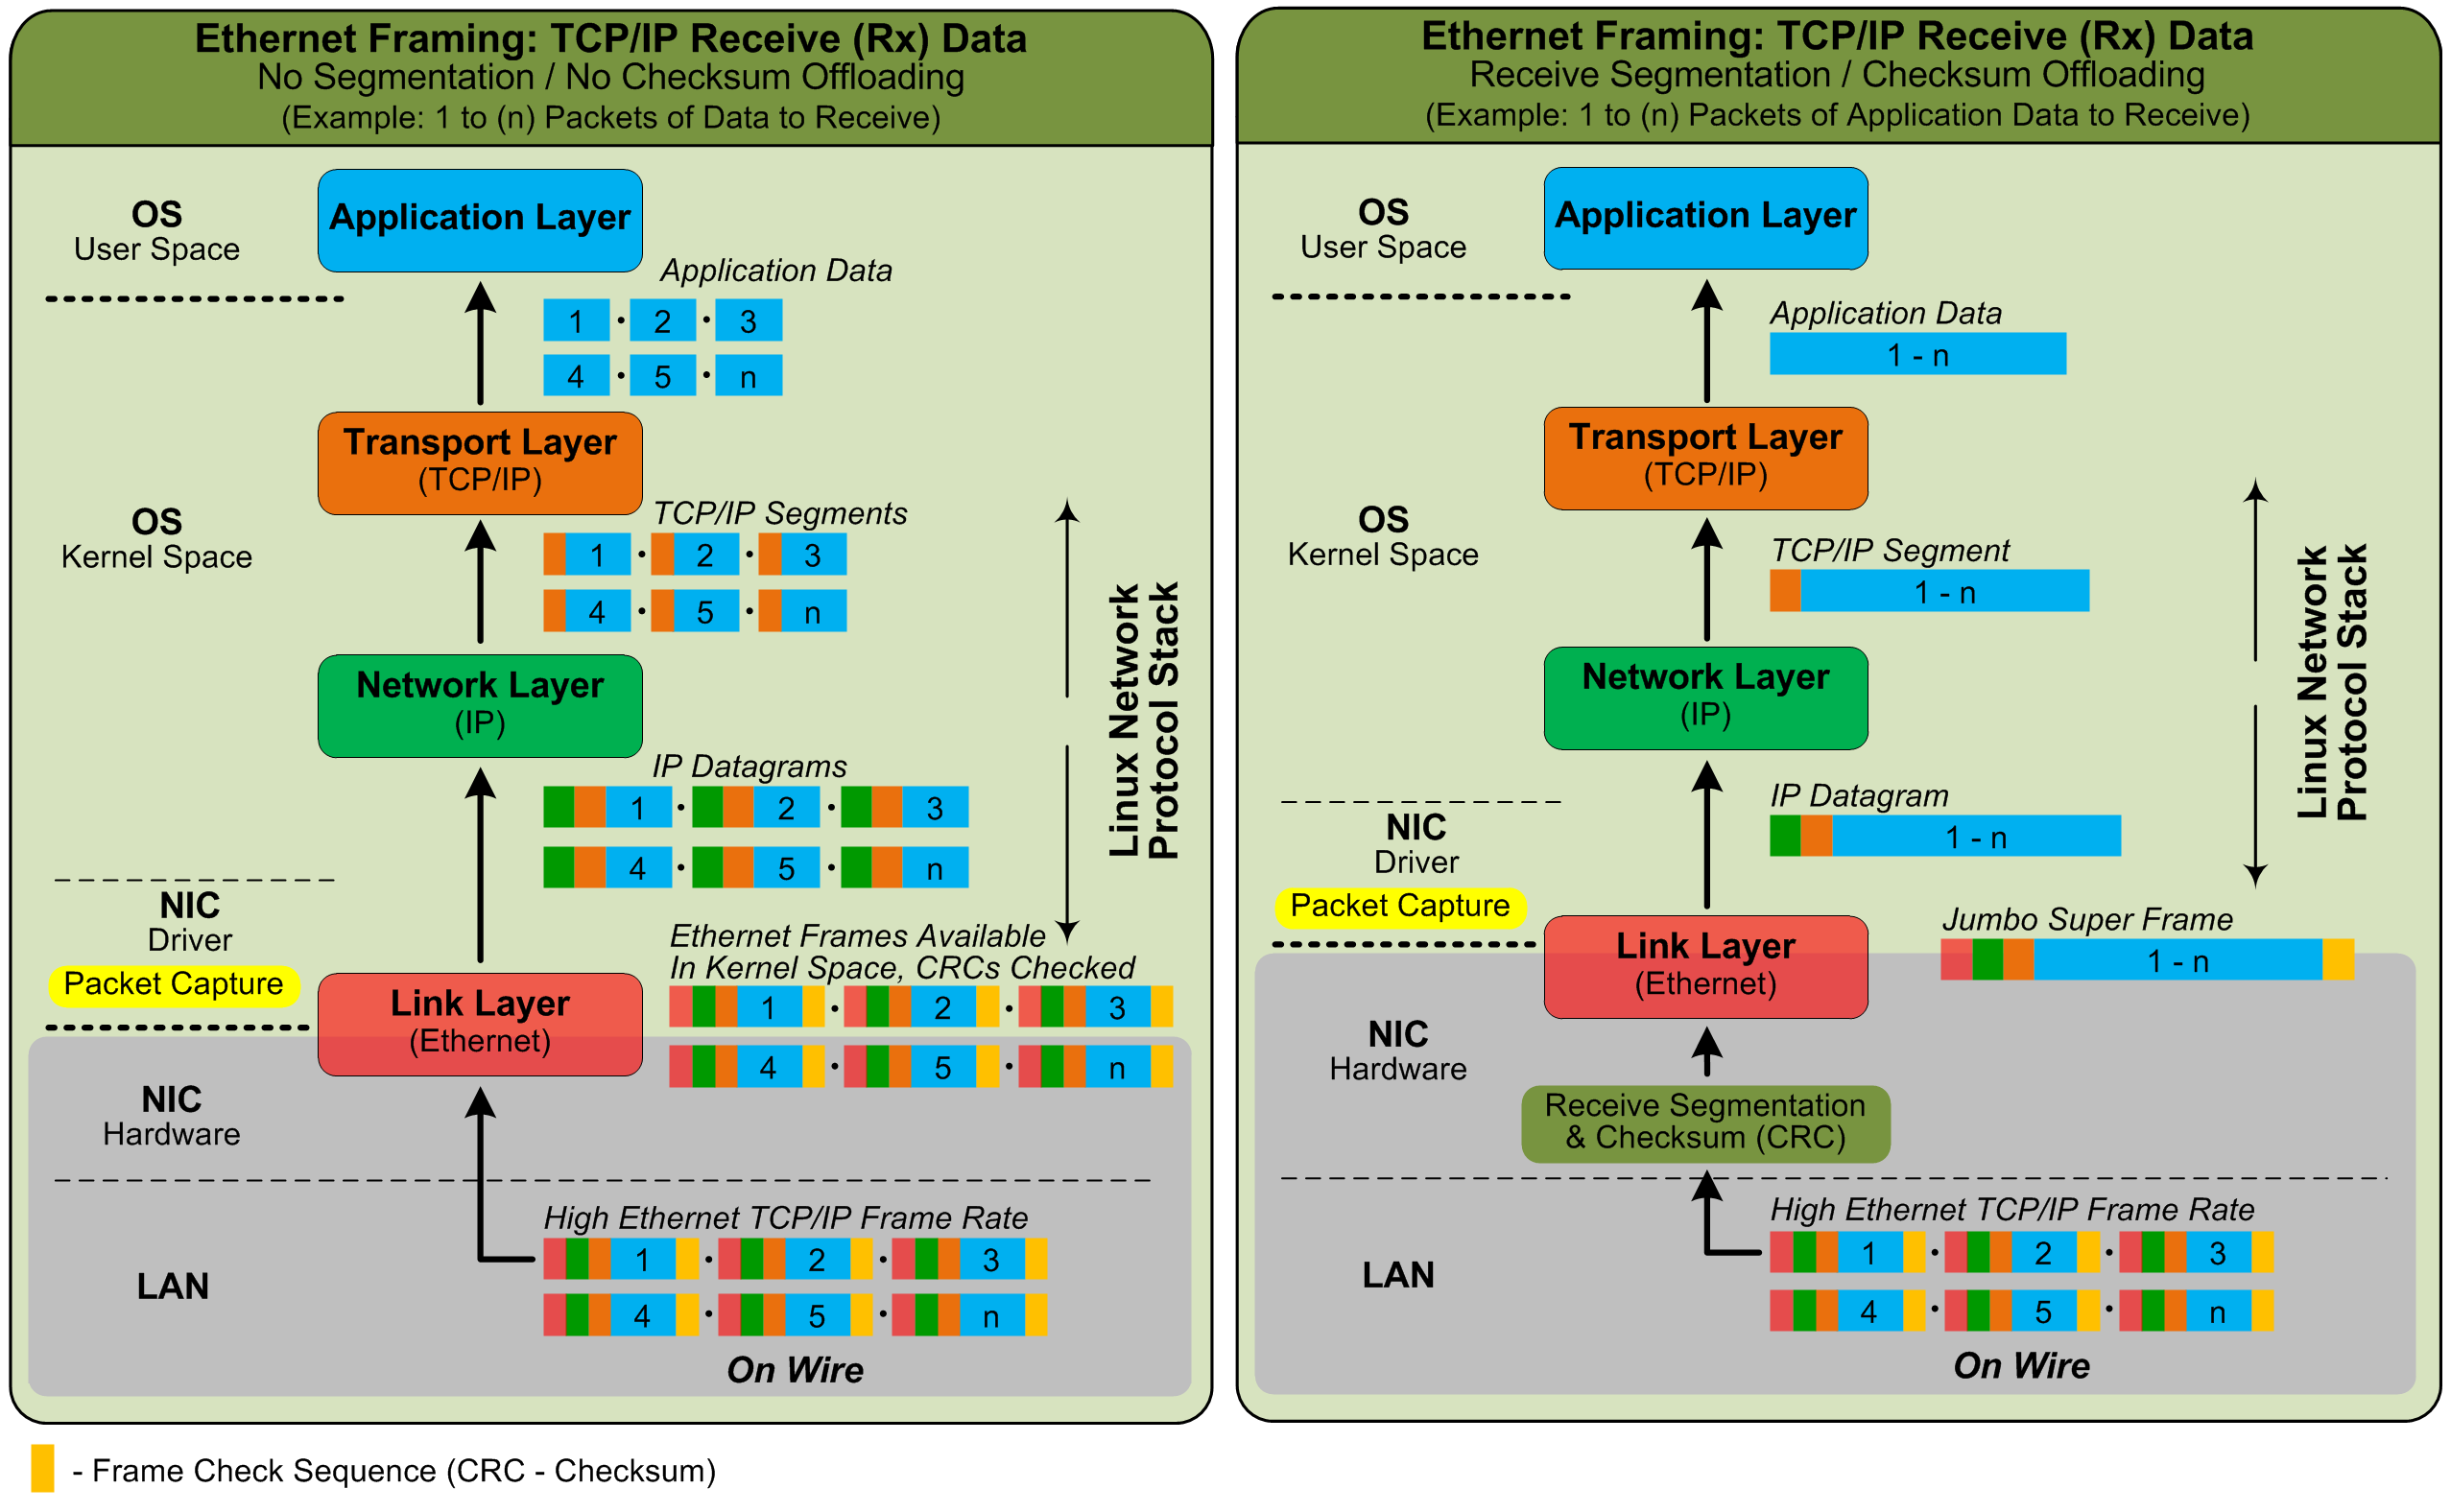
\includegraphics[width=15cm,keepaspectratio]{fig/rcv-offloads.png}
	\caption{Receive offloads (source:~\cite{nst-offloads})}
	\label{fig:linux-rcv-offloads}
	\bigskip
\end{figure}


%-----

%There are a number of advantages to doing things this way:
%vast numbers of interrupts can be avoided, incoming packets can be more efficiently processed in batches,
%and, if packets must be dropped in response to load, they can be discarded in
%the interface before they ever hit the network stack. Polling is thus a win for
%almost all situations where there is any significant amount of traffic at all~\cite{low-latency-ethernet-device-polling}.


%---





%quota is an integer that represents the maximum number of buffers that can be
%dequeued by the poll virtual function in one shot. Its value is incremented in
%units of weight
%For devices associated with non-NAPI drivers, the default value of weight is 64,
%stored in weight\_p at the top of net/core/dev.c. The value of weight\_p can be
%changed via /proc.
%For devices associated with NAPI drivers, the default value is chosen by the driv-
%ers. The most common value is 64, but 16 and 32 are used, too. Its value can be
%tuned via sysfs~\cite{understanding-internals}.


%%The input queue is managed by softnet_data->input_pkt_queue. Each input queue
%%has a maximum length given by the global variable netdev_max_backlog, whose value
%%is 300. This means that each CPU can have up to 300 frames in its input queue wait-
%%ing to be processed, regardless of the number of devices in the system.
%%sysctl -w net.core.netdev_max_backlog=250000
%NAPI devices use private queues, the devices can select the maximum length they prefer~\cite{understanding-internals}.



%%Similarly every complete transmission of an outgoing packet causes interrupt.

%---


%softirq - http://lwn.net/Articles/520076/
%the priority of network softirq handling to be raised on systems where networking needed realtime response


%-----


%---
%Jitter is unpredictable by default

%netperf

%---

%Protocol offload engines (ISO/OSI layers 2-4 implemented in HW)
%on Ethernet - %http://www.ics.uci.edu/~ccgrid11/files/ccgrid11-ib-hse_last.pdf
%Interrupt coalescing, Jumbo frames, HW checksum engines, Segmentation Offload engines

%Timestamp represents the time the frame was received and has a significant CPU cost~\cite{understanding-internals}.

